\section{\ivfprototype{} Implementation}
\label{implementation}

This section will go into the implementation details for the developed \ivfprototype{}.
Architecture, functions, data model, and the user interface design will be presented below.

The Rosemary architecture was fully reused, the only change is that neuroscience specific components were removed, as presented in figure \ref{fig:reuse-rosemary-architecture}.
On the level of code and structure, however, some changes were made to accommodate the \ivfprototype{} functionality.

Due to previously mentioned time restrictions not all functions that were discovered could be implemented.
A selection is made based on the programmers opinion what would be most profitable for a prototype system, considering that the prototype has to appeal to a wide variety of users.
Most importantly the key stakeholders in the brainstorm (section \ref{brainstorm}) but also, for example, clinic management.
Functions that were deemed less important during the brainstorm were excluded from consideration.
The selection is shown in figure \ref{fig:functions-workflow}: the implemented functions have a dashed border.

The system's critical functions have been implemented such as: user registration and management, data requests and acquisition.
To give the system eye-catchers and illustrate its potential value, the data audit has been implemented through so-called placeholders, \ie{} functions have pre-defined responses and do not work with the `live' data.
Also, different representation methods for data have been explored, for example: raw data, aggregated data, data in a graph.
This will be further explained in the user interface implementation details.

Where in the Rosemary data could be an image with its metadata in the \ivfprototype{} it is a pregnancy and its metadata.
Because data requests are selections on the \projectdata{} there needs to be a way to allow access \emph{only} to the selected items (headers).
A request explicitly defines which headers are needed.
Data headers can be any information that is available for a pregnancy, examples are: age mother, type of treatment, birth weight, etc.
After a request has been approved the system creates a new subset (\ie{} a workspace) which is accessible by the requesting researcher.
Figure \ref{fig:dataset-example} shows the difference between a workspace with access to \emph{all} the data versus one with only four headers for the exact same pregnancy.

\begin{figure}[ht]
	\centering
	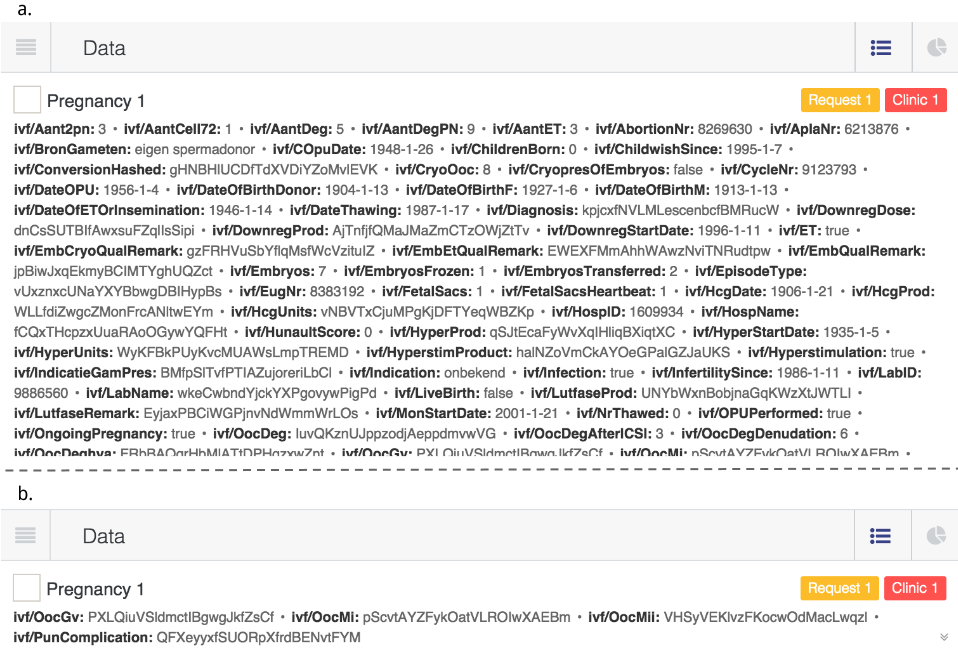
\includegraphics[width=1.0\linewidth]{images/datasets-example-edit}
	\caption{
		Example of the full \projectdata{} (a) versus a restricted view (b).
		The restricted view shows exactly the same pregnancy but only the requested (and accessible) four data headers are displayed.
	}
	\label{fig:dataset-example}
\end{figure}

\paragraph{Functionality: back-end and front-end}
The most notable changes to existing back-end code were in the security classes and data handling.
Rosemary already supports basic user management, where access to the system is provided based on the user account.
However the system needed to be extended with user roles for more fine-grained access control, \ie{} a distinction between researchers, administrators, and committee members.
To execute this control the system requires these roles to be readable and actionable (\ie{} the system can act upon a specific role).
This is reflected in the {\tt Security} class which now supplies this information.

Even though security considerations are a big part of the requirement analysis (see section \ref{security}), it does not show itself that clearly in the system implementation.
Most of the security measures were taken during the data gathering steps.
Because the decision was made to have a fixed dataset for the system a lot of the discussed security measures do not need to apply anymore as described in section \ref{security-summarisation-analysis}.
Provenance is not supported due to time restrictions.

Data header filtering based on the workspace is not something that was available therefore the data handling had to be changed.
The front-end asks for data from the back-end based on the logged-in user and the workspace they are trying to access.
To make sure data is handled safely the back-end has to filter the data before passing it on to the front-end.
Based on the workspace details (\ie{} which headers have been requested and approved) the back-end filters the \projectdata{}, the filtered (sub)set is then displayed.

Lastly, the RESTful API was supplemented with (read, store, edit, delete) functions for newly introduced data concepts (\eg{} data requests).
These concepts will be described below.

\paragraph{The data model}
Unlike the architecture the data model needed alterations.
These can be divided into changes to already existing objects and additions of new objects.

To make data filtering possible support for limiting data headers had to be added.
This is achieved by tagging the {\tt Datum} objects with a {\tt WorkspaceTag}.
The {\tt WorkspaceTag} object was extended with a set that holds the data headers that were requested and should be accessible.
Back-end functions for {\tt Datum} objects check the tag and filter the available data.

Rosemary does not differentiate between different types of workspaces. 
The \ivfsystem{} has three types of  workspaces: the \emph{master} workspace containing the whole \projectdata{}, clinic workspaces containing data specific to a clinic, and request workspaces.
This is reflected by adding a workspace type field to the {\tt WorkspaceTag} object.

To support data requests the following five objects were added to the model: {\tt Research}, {\tt Approval}, {\tt Data Request}, {\tt DownloadNotif}, {\tt RequestNotif}.
The two notification objects are used to determine how notification information is displayed in the front-end. 
They both inherit from the {\tt Notification} object, which remains unchanged compared to Rosemary.
This means that the methods used to extract information are standardised, and that new notification objects can directly be used in the system without further need for customisation.

The other three objects are related to each other: each {\tt Research} contains an {\tt Approval} object and a {\tt Data Request} object.
These related objects are used to capture data regarding the request progress.
The {\tt Data Request} contains the requested headers.
The {\tt Approval} keeps record of which committee members  need to give permissions, and which votes were already cast.
Lastly, the {\tt Research} object is used to capture information used to base a voting decision on, \eg{} research question, study description, etc.

\paragraph{User interface design}
In this project there was no time available for a user-centred design approach, where prototypes are iterated until the best design solution is achieved.
The front-end design was strongly based on the existing Rosemary UI style, and for each new function a page was created where necessary.

Figures \ref{fig:wireframe-layout} and \ref{fig:wireframe-basket-layout} show the wireframe representations of the implemented layout for the data management in the \ivfprototype{}.
The menu is shown on the left and the notifications are on the right. 
When a user browses pages only the middle part updates (\ie{} web application feel).
The user may switch between pages through the menu. 
All available functions have their own menu button (\eg{} request, workspaces, messages).
All accessible workspaces for a user are listed: these can be any of the three types mentioned earlier (\ie{} master, clinic, request).

Changes to the Rosemary design included the addition of a data summary panel, removal of superfluous filter possibilities, and the addition of a download button to the basket.
The filter panel embodies the searching functionality of the gateway.
The basket supports selection and acquisition (downloading), while the summary and data components handle the different views on data.

\begin{figure}[hb]
	\centering
	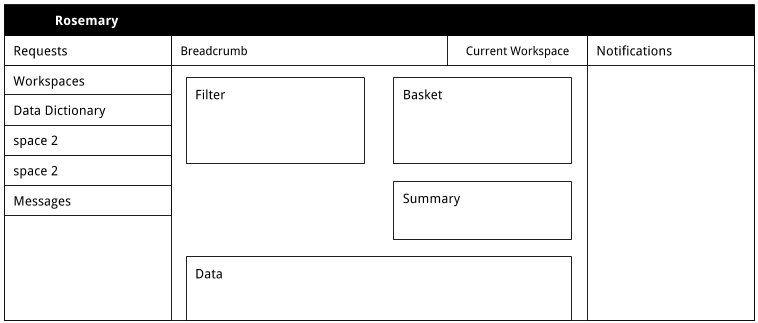
\includegraphics[width=1.0\linewidth]{images/evaluation-layout}
	\caption{
		ireframe representation of the UI layout, showing the data management features: filter, view, select.
	}
	\label{fig:wireframe-layout}
\end{figure}

\begin{figure}[hb]
	\centering
	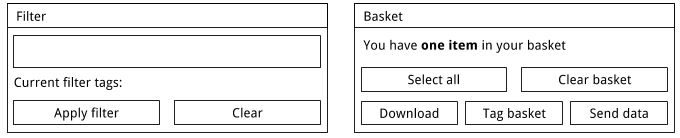
\includegraphics[width=1.0\linewidth]{images/evaluation-basket-layout}
	\caption{
		Wireframe representation of the UI for filter and basket layout, showing the search and select data management tools.
		(Details of the filter and basket blocks in figure \ref{fig:wireframe-layout}).
	}
	\label{fig:wireframe-basket-layout}
\end{figure}